\documentclass[12pt]{article}
\usepackage[hmargin=1in, vmargin=1in]{geometry}
\usepackage{fancyhdr}
\usepackage{setspace}
\pagestyle{fancy}
\usepackage[small]{caption}
\usepackage{lastpage}
\usepackage{listings}
\usepackage{graphicx}
\usepackage{verbatim}
\usepackage{url}
\DeclareGraphicsExtensions{.png}

% Custom colors
\usepackage{color}
\definecolor{deepblue}{rgb}{0,0,0.5}
\definecolor{deepred}{rgb}{0.6,0,0}
\definecolor{deepgreen}{rgb}{0,0.5,0}
\definecolor{grey}{gray}{0.9}


\lstset{
    tabsize=2,
    breaklines=true,
    showstringspaces=false
    backgroundcolor=\color{grey},
    basicstyle=\ttfamily\scriptsize,
}


\def\author{Jacques Uber}
\def\title{Assignment 2: Contributing to Django}
\def\date{\today}

\fancyhf{} % clear all header and footer fields
\fancyhead[LO]{\author}
\fancyhead[RO]{\date}
\renewcommand{\headrulewidth}{0pt}
% The weird spacing here is to get the spacing of \thepage to be right.
\fancyfoot[C]{\thepage\
                    / 3}

\setcounter{secnumdepth}{0}
\setlength{\parindent}{0pt}
\setlength{\parskip}{4mm}
\linespread{1}
% Talk about how the hinge works and where the power switch it relative to how the hinge swings.
% Pictures:
%   Use copyright: Name, Year
% Get rid of value language
%
% OO: Wednesday 9-12
%
\begin{document}
%\fancyhead[CO]{\title}
\begin{center}
\underline{
\large{\title}
}
\end{center}
\singlespacing

\section{Django part 2.}
For my second contribution assignment, I attempted to make a another contribution to the Django
project. The attempt failed. I tried to work on ticket \#16731: 'startswith and contains
doesn't work with F expression'. I spent a few days tinkering with the issue and tried to diagnose
the it. I found that while the code causing the bug was easily identifiable, coming up with a
solution was not easy. I decided that I could not contribute a patch or even a helpful
suggestion about how to fix the bug. But, I did make a contribution to the ticket, which
identified an unmentioned way to trigger the bug. Here is a screen-shot of that comment:

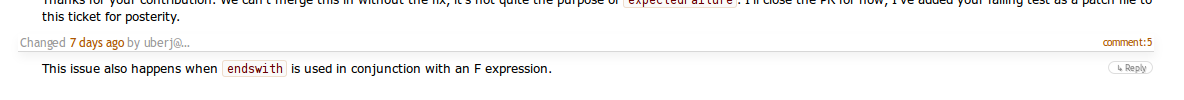
\includegraphics[width=6.5in]{django_fail}

After failing with that, I decided to look in the easy pickings section of Django's issue tracker. I
noticed that \emph{most} of the tickets that would be good for a new contributer already included a
patch or pull request. I narrowed my search to tickets marked 'easy pickings' that also did not
have a patch; I found there were three tickets that met these conditions. All three tickets
were over 4 years old and not anything I could contribute to.

\subsection{Weechat}
Weechat is an IRC client. I use it on a daily basis and there is a bug/feature with the UI that
bothered me, so I decided to see if I could try to report the issue and even try to fix it. I
first searched their bug tracker for a report of the issue I was having and after I didn't find
anything I searched their mailing list archives -- I didn't find anything. I next went to \#weechat
on irc.freenode.net to ask about my issue, here are the chat logs:

\begin{lstlisting}
17:57    uberj   when I put a url into weechat that spans
                 multiple lines only the top line is underlined when I hover my
                 mouse over it.  Is there an open issue for that?
17:59    uberj   because I don't see one on this page
                 (http://savannah.nongnu.org/bugs/?group=weechat)
18:04    faen    it's a known problem, but not something weechat can do much about
18:05    Nei     the underline is generated by your terminal, which has no clue
                 about linebreaks and stuff
18:05    uberj   faen: don't get me wrong, I like weechat, but irssi handles with fine.
18:05    uberj   s/with/this/
18:05    faen    uberj: yes, because irssi doesn't have nick alignment or sidebars
18:05    faen    (by default)
18:06    Nei     irssi cant do vertical stuff, and doesnt use ncurses
18:06    uberj   ah
18:06    Nei     irssi makes the url on a single line, which wraps naturally at
                 your terminal border
18:06    uberj   so if I added a side bar or something, it wouldn't work anymore?
18:07    Nei     if you added a sidebar to irssi it would equally break
18:07    uberj   that makes sense
18:07    grawity current terminals just cannot be told that there are multiple
                 columns of text
18:07    grawity unfortunately
\end{lstlisting}

Weechat seemed like a bust. The issue I wanted to fix seemed to be unfixable.


\section{Getting Desperate}

I decided that contributing something useful like a bug report to any project was going to get
tricky because I was running out of time. So I decided to look for typo's in documentation. Because I
suck at spelling I decided to rely on firefox to find typo's for me. My strategy was to go to a page
full of documentation and run this javascript in the browser:


\begin{lstlisting}
    document.body.contentEditable='true'; document.designMode='on'; void 0;
\end{lstlisting}

This causes an entire page to become editable and thus be spell-checked by firefox.

\section{Finding a bug in Firefox}
When you visit a page that contains text that will be spell-checked, for example in a \emph{textarea}
tag, firefox will stop checking for misspelled words after it finds 375 mistakes. I found a bug! --
so I filed a bug:

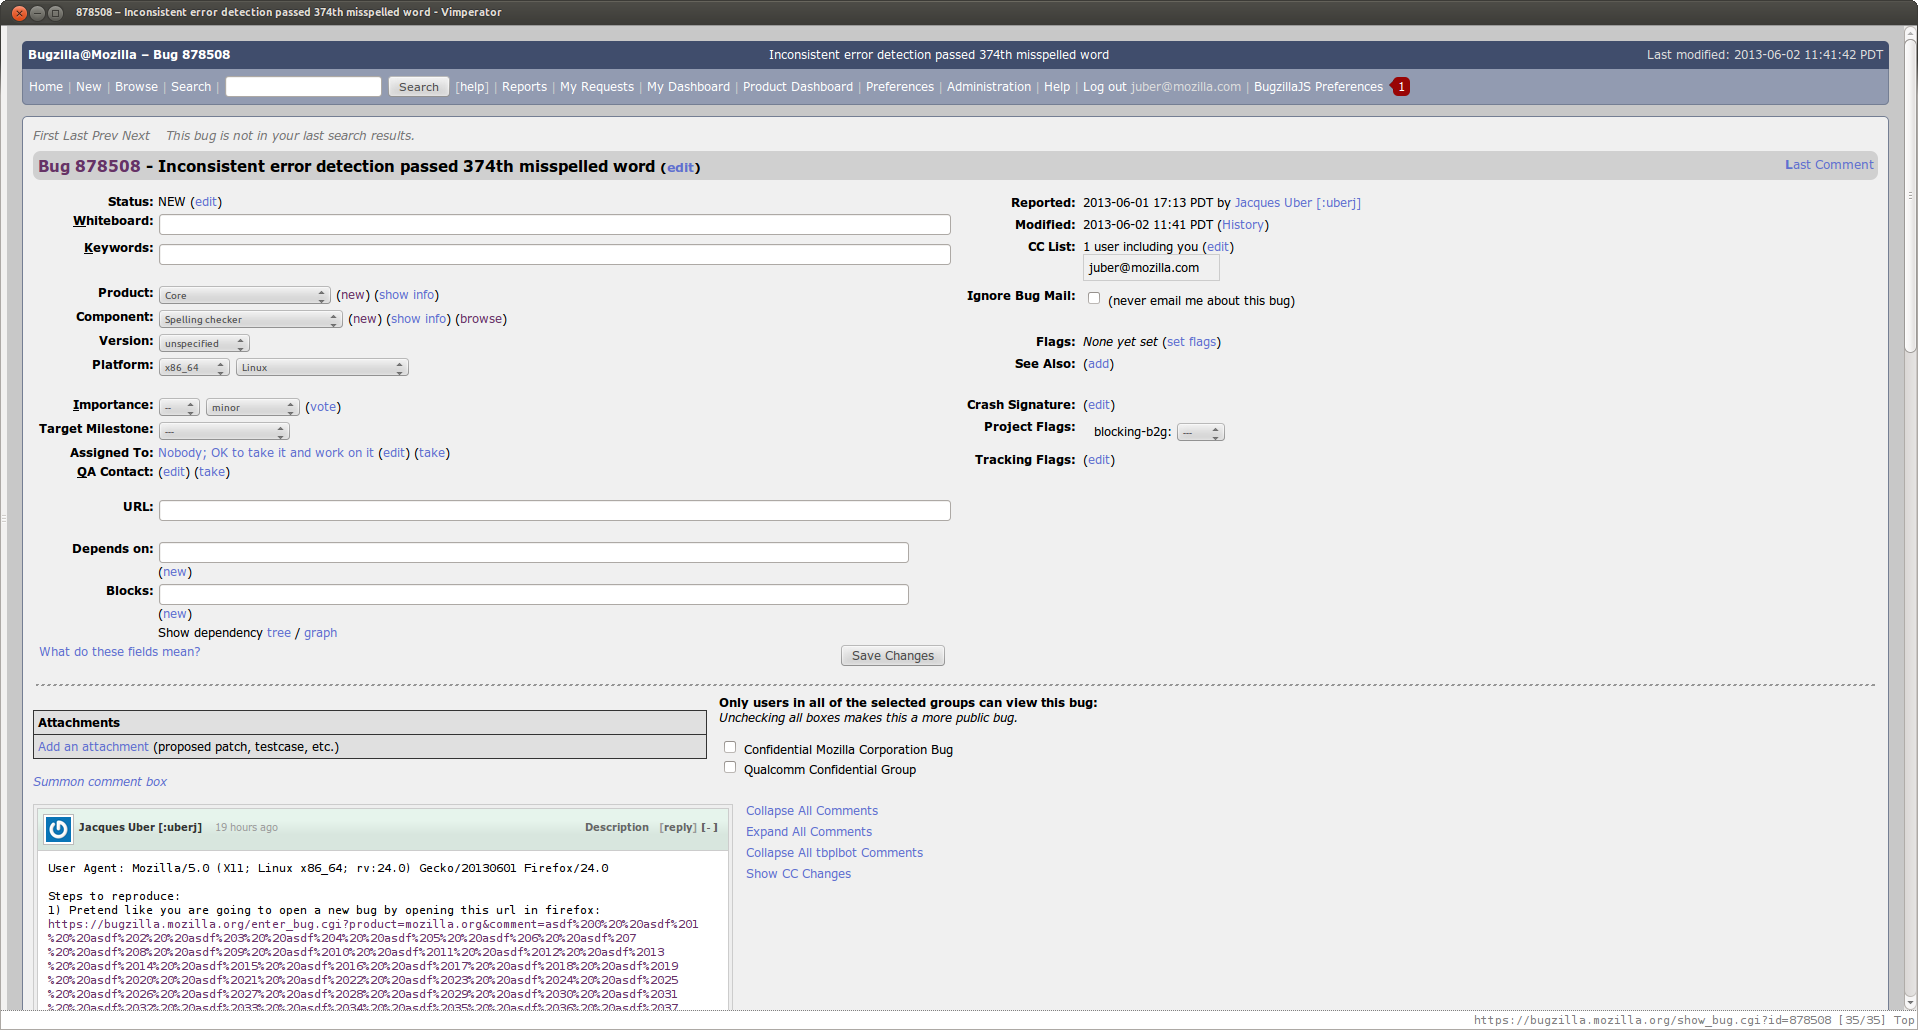
\includegraphics[width=6.5in]{cs419_part1}


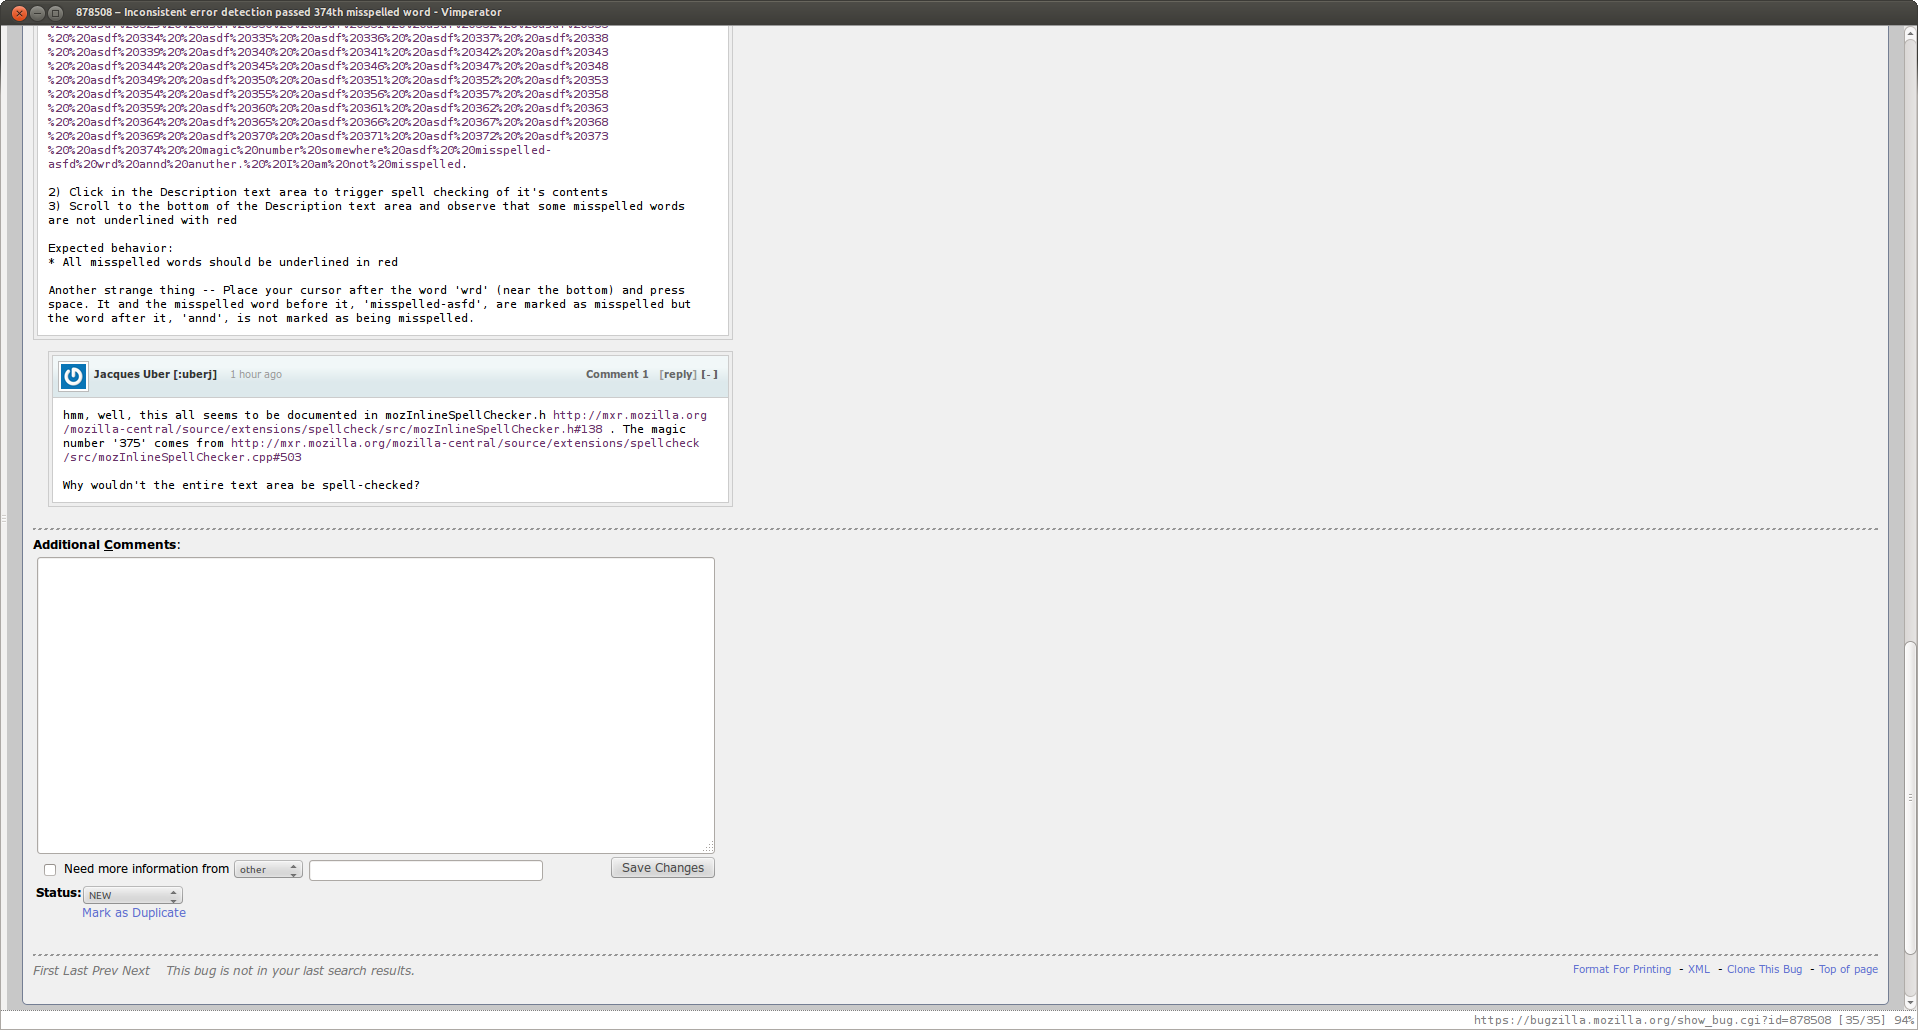
\includegraphics[width=6.5in]{cs419_part2}

\subsection{My bug was a workaround in another bug}

It turns out that the behavior I thought was a bug is really a workaround for poor performance.
Shortly after I filed the bug, a developer named Robert Longson, commented on the bug I filed. His
comment was 'See bug 324521 for why.'. Bug 324521 explained that spell-checking very large files
with a lot of text causes firefox to hang.

\end{document}
